\documentclass[letterpaper]{article}
\usepackage[submission]{aaai2027}
\usepackage[hyphens]{url}
\usepackage{graphicx}
\urlstyle{rm}
\def\UrlFont{\rm}
\usepackage{natbib}
\usepackage{caption}
\usepackage{booktabs}
\usepackage{amsmath,amssymb}
\frenchspacing
\pdfinfo{/TemplateVersion (2027.1)}

\newcommand{\pp}{\,pp}
\title{Selection Purity Is Not a Sufficient Proxy for Transfer Utility: Auditing Joint Model and Data
Heterogeneity in Language-Model Adaptation}
\author{Anonymous Authors}
\affiliations{Anonymous Affiliation}

\begin{document}
\maketitle

\begin{abstract}
Federated language-model adaptation is often evaluated with homogeneous
client architectures or task-consistent client data.  We study these two
forms of heterogeneity jointly: different decoder-only model families train on mixtures of
useful, conflicting, and off-task examples.  Our serialized protocols use real
checkpoints, hashed manifests, clean-safety gates, official test sets and disjoint evaluation splits, and
raw artifact hashes.  On AG News, tokenizer-agnostic distillation from routed
heterogeneous clients is \(0.56\) percentage points worse than a matched
public-anchor-only server and costs \(2.01\times\) the wall time.  A
post-observation check on the same test repeats the negative direction in all
five new seeds (mean \(-0.80\pp\)).  On a separately frozen six-class
TREC official evaluation, five seeds show no clear accuracy gain (\(+0.40\pp\), 95\% seed
interval \([-1.74,+2.54]\pp\)), while ECE falls by 0.0373 descriptively.
After observing that result, a post-primary same-test mechanistic ablation with ten new seeds
finds severe unfiltered transfer above clean transfer by \(1.58\pp\)
(Holm \(p=.015\)), whereas the complete routed intervention is \(1.42\pp\)
lower (Holm \(p=.0074\))
while lowering observed ECE.  On GSM8K, an
independently anchor-trained teacher used only to rank supplied answers
improves a Qwen client by \(3.34\pp\) under severe contamination.  Positive
severe differences for SmolLM2 and TinyLlama fail a predeclared,
post-observation Holm-corrected cross-family gate.  Oracle-rate Co-Teaching is
nonuniform on controlled and natural weak-label mixtures; both natural-noise
development gates fail, so their test splits are not evaluated.  Our evidence is diagnostic
rather than algorithmic: routed transfer has no consistent accuracy benefit
across two server tasks; both show lower observed ECE, a descriptive secondary
pattern.  In contrast,
training-only selection helps one local Qwen setting without establishing
beneficial federated transfer or cross-family stability.
\end{abstract}

\section{Introduction}
Federated fine-tuning promises to adapt language models without moving private
client text.  Two assumptions make this problem look easier than it is.
First, many methods assume compatible client parameters even though deployed
models can differ in width, tokenizer, and architecture.  Second, evaluations
often assume that a participating client's data is uniformly useful for the
server task.  Real client corpora can instead contain a mixture of useful
examples, unrelated tasks, and responses that directly conflict with the
target capability.

These axes interact.  Parameter-space averaging may be undefined across model
families, but moving to logits or probabilities only solves the interface
problem; it does not establish whether transferred signals optimize the target
server metric.  Conversely, a local data
filter that works for one model family may exploit architecture-specific loss
scales and fail on another.  We ask: \emph{which conclusions survive when
model-family and within-client data heterogeneity occur together?}

We make one evaluation contribution centered on the distinction between
selection purity, probability quality, and downstream utility.  We factor heterogeneous
adaptation into local selection, canonical client-to-server transfer, and a
public-anchor-only server control.  Two finite-label server tasks instantiate
this audit; open-answer and natural-weak-label studies test the boundary of the
local-selection stage.  We report conditional and negative outcomes with
explicit pre-/post-observation scope, paired uncertainty, multiplicity
control, cost, and content-addressed artifacts.  This is a controlled
diagnosis of where selection metrics and heterogeneous-transfer utility diverge, not a new optimizer or
privacy mechanism.
Figure~\ref{fig:framework} separates the server-transfer and local-selection
branches.

\begin{figure*}[t]
\centering
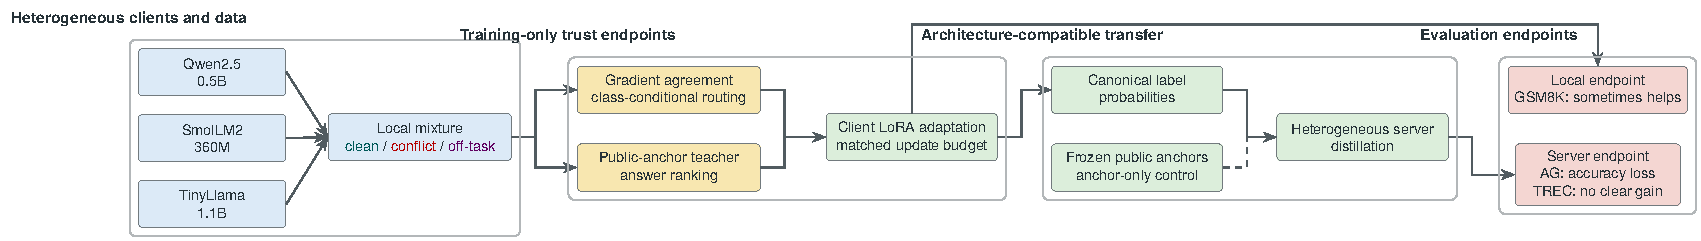
\includegraphics[width=\textwidth]{figures/framework.pdf}
\caption{Evaluation framework.  Heterogeneous client models train on mixtures
of clean, conflicting, and off-task data.  Routed client probabilities are
transferred in the AG News and TREC server experiments; Co-Teaching and teacher
ranking are local-adaptation controls.  The public-anchor-only server is the
matched transfer control, and local gains are not evidence of beneficial
federated transfer.}
\label{fig:framework}
\end{figure*}

\section{Related Work}
\paragraph{Federated PEFT and model heterogeneity.}
FedAvg aggregates compatible client parameters \cite{mcmahan2017fedavg}, while
FedMD and FedDF use public-data distillation to relax the shared-architecture
assumption \cite{li2019fedmd,lin2020feddf}.  LoRA makes adaptation economical
by training low-rank updates \cite{hu2022lora}, but factor exchange does not by
itself resolve architectural incompatibility.
FedBiOT compresses a server LLM for client-side adaptation
\cite{wu2024fedbiot}.  HetLoRA supports heterogeneous client LoRA ranks
\cite{cho2024hetlora}, while FLoRA avoids cross terms through stacking
\cite{wang2024flora}.  FedMKT transfers knowledge between server LLMs and
client SLMs \cite{fan2025fedmkt}.  These works establish that heterogeneous
LoRA and cross-size knowledge transfer are not new.  We test a distinct
stress setting in which heterogeneous clients are also internally
contaminated.
Our severe-unfiltered arm is a FedMD/FedDF-style uniform canonical-probability
ensemble-distillation control adapted to decoder-only verbalizer classes; it
is not an exact reproduction of either algorithm.

\paragraph{Noisy labels and data selection.}
The early-learning behavior of deep networks motivates small-loss selection
\cite{arpit2017memorization}.  Co-Teaching exchanges peer-selected small-loss
examples \cite{han2018coteaching}; trusted clean data can also estimate noise
corrections \cite{hendrycks2018trusted}.  Superfiltering shows
that a weak language model can select instruction data for a stronger model
\cite{li2024superfiltering}.  Delora decouples a dual-LoRA noisy-label detector
from downstream PEFT \cite{yuan2025delora}, and FedClean performs clean-sample
selection, multi-stage finite-class relabeling, and robust aggregation
\cite{jiang2025fedclean}.  Thus our public-anchor teacher score is a simple
diagnostic endpoint.  Delora and FedClean do not directly specify unbounded
numeric relabeling or aggregation across incompatible model parameters; we
report this interface incompatibility rather than claiming to outperform
them.

\section{Problem Setting}
Clients \(c\in\{1,\ldots,C\}\) own decoder-only models \(f_c\), tokenizers
\(\tau_c\), and datasets \(D_c\).  The server model \(f_s\) may have a
different architecture and tokenizer.  A client dataset is a mixture
\[
D_c=D_c^{\mathrm{clean}}\cup D_c^{\mathrm{conflict}}
    \cup D_c^{\mathrm{off}},
\]
where conflicting examples retain a target-task input but provide an
incorrect answer, and off-task examples use a different task interface.
Clients and server share a small public target-task anchor set \(A\).

For architecture-agnostic classification exchange, client \(c\) transmits a
probability vector over the canonical label set for every anchor input.  The
client score vector contains token-normalized candidate-answer losses
\(\boldsymbol\ell_{ci}\), giving
\(q_{ci}=\operatorname{softmax}(-\boldsymbol\ell_{ci})\) for anchor \(x_i\).
The server uses \(\bar q_i=C^{-1}\sum_cq_{ci}\), computes its own canonical
probabilities \(p_s\), and minimizes
\(\mathcal L_s=\lambda_A\operatorname{CE}(y_i,p_s)+
\lambda_D\operatorname{CE}(\bar q_i,p_s)\).
The anchor-only control sets \(\lambda_D=0\); routed transfer uses the frozen
\(\lambda_D\).  This interface is compatible by construction, but its utility
depends on client data quality.

\section{Training-Only Trust Endpoints}
\subsection{Class-conditional gradient routing}
For a labeled example \(z=(x,y)\), let \(g(z)\) be the gradient of its causal
answer loss with respect to local LoRA parameters and let \(a_y\) be the mean
gradient of public anchors from class \(y\).  Their agreement is
\[
s_g(z)=\frac{g(z)^\top a_y}{\lVert g(z)\rVert\lVert a_y\rVert}.
\]
Let \(P(v_i)\in[0,1]\) denote the average-tie percentile rank of value \(v_i\)
within client \(c\), with lower values ranked first.  For target-task examples,
the inconsistency margin is \(m(z)=\ell_y(z)-\min_k\ell_k(z)\); off-task
examples receive one plus the largest observed target-task margin.  The risk is
\[
R(z)=\tfrac13\{P(-s_g(z))+P(\ell(z))+P(m(z))\}.
\]
Because raw cosine scales differ by model family, the routing gate uses the relative statistic
\[
r_c=\frac{Q_{0.25}(\{s_g(z):z\in D_c\})}
          {\max[Q_{0.25}(\{s_g(a):a\in A\}),10^{-12}]}.
\]
The gate triggers when \(r_c<0.8\); otherwise all examples are retained.  A
triggered client keeps the lowest-risk
\(\max(1,\operatorname{round}(0.5|D_c|/K))\) examples per claimed target
class, with source ID breaking ties; off-task examples have no claimed class
and are excluded.  Zero gradients are handled by the clamped cosine
denominator.  Thresholds and quotas were chosen on development data and fixed
before the corresponding official-test runs.  Clean-versus-conflict annotations
are audit-only and never enter the score.  Off-task membership is known from
the explicit task interface; such examples have no claimed target class and
are excluded whenever the gate triggers.

\subsection{Public-anchor teacher ranking}
Open numerical answers do not have a small canonical class set.  We train an
independent teacher \(f_T\) only on \(A\) and score a supplied pair
\(z=(x,\widetilde y)\) by token-normalized answer loss,
\[
s_T(z)=-\frac{1}{|\widetilde y|}
       \log p_{f_T}(\widetilde y\mid x).
\]
After a numerical-interface check, the client retains the \(K\) lowest-loss
examples and performs the same number of optimizer steps as the unfiltered
baseline.  No teacher parameter, hidden state, client validation label, or
test example is used.  The scalar endpoint is comparable across client model
families, but requires an additional model and serial candidate scoring.

\section{Experimental Protocol}
\paragraph{Stage A: topic classification.}
AG News is the four-way target task and IMDb supplies real off-task text
\cite{zhang2015agnews,maas2011imdb}.
Conflicts use a deterministic non-identity label permutation.  A frozen
manifest separates 256 public anchors, 800 development examples, disjoint
client pools, and the full 7,600-example official test.  Clients are
Qwen2.5-0.5B, SmolLM2-360M, and TinyLlama-1.1B; the server is
Qwen2.5-1.5B.

\paragraph{Stage A2: independent question classification.}
TREC-Coarse provides a six-way answer-type task \cite{li2002question}; IMDb
remains the off-task source.  Exact duplicate training lines are removed by
raw-line hash before a balanced allocation of 72 anchors, 72 development
questions, and three disjoint 120-question client pools.  Each client class
contributes 8 clean, 8 cyclic-conflict, and 4 off-task slots.  The complete
500-question official test is evaluated over five seeds.  The task, manifest,
runner, full arguments, canonical \([72,6]\) probability payloads, and
serialized wire payloads are content-addressed.  The model families, two
rounds, update budget, and routing thresholds match Stage A.
The parent primary protocol was frozen after instrumentation repairs and before
its official evaluation; those repairs and invalidated smoke runs are recorded
in its protocol history.  The later four-arm protocol explicitly records prior
test access and its own audit-counter repair before any retained full aggregate.

\paragraph{Stage B: numerical reasoning.}
GSM8K supplies target questions and SQuAD supplies off-task QA
\cite{cobbe2021gsm8k,rajpurkar2016squad}.  Conflicts use
deterministically rotated final numeric answers.  The primary manifest
separates public anchors, 512 development questions, and three client pools.
Official evaluation uses all 1,319 test questions.  After observing the
primary phase, we froze a disjoint post-primary evaluation split of 1,024
training-split questions after excluding
every anchor, development, and client-pool index; 4,913 unused questions
remain.  Answers are greedily generated, decimal-normalized, and scored by
exact match.
The client checkpoints are documented by their family reports
\cite{qwen2025technical,benallal2025smollm2,zhang2024tinyllama}.

\paragraph{Controls and statistics.}
Within each server task, comparisons match server initialization, public
anchors, server optimizer steps, prompts, and seed.  The original AG News
primary and seed replication execute shadow unfiltered clients but set
\(\lambda_D=0\), so their recorded probability payload is unnecessary to the
server rather than absent.  The TREC anchor and the later AG four-arm runner
omit the client path.  Cost ratios are therefore protocol-specific and do not
share one end-to-end work definition.  Local-selection comparisons match client
optimizer steps.  Each run-level protocol is serialized before its corresponding
execution; this does not make later phases globally preregistered once an
earlier phase has accessed the same benchmark test.  We report paired
differences and descriptive Student-\(t\) intervals over three seeds; these
intervals characterize seed-to-seed variation, not task- or sample-level
uncertainty.  TREC uses a two-sided paired test over five designated official seeds because
either direction is reportable; the directional improvement tests below are
one-sided.  Its post-primary ablation uses ten new common seeds and exactly
three adjacent two-sided accuracy contrasts with one joint Holm correction;
secondary metrics are descriptive and the already accessed test is disclosed.
Declared families of primary contrasts use Holm correction.  Raw JSON records
carry evidence labels, model and manifest hashes, split scope, wall time, and
peak GPU allocation; corpus-file hashes are present in the natural-label runs.
All other reported improvement tests are one-sided paired Student-\(t\) tests over
seed-matched differences.  Holm correction is applied separately to the six
AG News Co-Teaching contrasts, two cross-family GSM8K contrasts, nine
family-by-severity secondary contrasts, and three contrasts within each
natural-language development study.

\paragraph{Natural weak-label protocol.}
The COMPRISE Hausa and Yoruba topic datasets provide distant-supervision labels
aligned with released clean training labels, plus separate clean development
and test splits.  Before training, we froze the measured disagreement rate as
Co-Teaching's oracle forget rate, three new seeds per language, and a release
gate requiring nonnegative mean gains for every family and at least one
Holm-adjusted improvement.  Clean training labels determine the single global
oracle forget rate and support selection audits; per-example clean labels do
not enter scoring, selection, or the training objective.  A failed gate
forbids test evaluation.

\paragraph{Metrics and optimization.}
For AG News and TREC, class scores are negative token-normalized answer-suffix losses;
we report accuracy, macro-F1, the true-label suffix loss, and 10-bin ECE from
the resulting canonical probabilities.  GSM8K uses decimal-normalized exact
match; natural-label studies use accuracy with macro-F1 as an imbalance audit.
TREC additionally reports normalized canonical class NLL.  All adapters target query/value projections with LoRA rank 4, scale 8, and no
dropout, optimized by AdamW.  The AG holdout uses two rounds of 40 client and
40 server steps (batch 8; server learning rate \(10^{-4}\)); GSM8K uses 40
steps at batch 4 and \(10^{-3}\); natural-label runs use 256 steps at batch 8
and \(10^{-3}\).  Frozen JSON protocols contain the remaining generation,
length, and selection settings.

\section{Results}
\subsection{Server distillation yields task-dependent accuracy utility}
At development seed 42, severe AG News mixtures reduce local accuracy by
21.75--25.88 points across the three client families.  The relative router is
clean-safe in that three-family check; across Qwen seeds 42--44 it improves
severe local accuracy by \(+3.37\) to \(+30.00\pp\).  This local improvement
does not translate to the server endpoint.

\begin{table}[t]
\centering
\scriptsize
\setlength{\tabcolsep}{3pt}
\caption{Server results. Accuracy is mean \(\pm\) SD; Macro-F1 and ECE are
seed means. Rows below the rule are the post-primary reused-test TREC ablation
with ten new seeds.}
\begin{tabular}{llccc}
\toprule
Task & Method & Accuracy & Macro-F1 & ECE\\
\midrule
AG News & Anchor-only & \(84.34\pm0.62\) & 84.28 & 0.054\\
AG News & Routed & \(83.78\pm0.54\) & 83.67 & 0.016\\
TREC & Anchor-only & \(80.72\pm1.41\) & 77.65 & 0.068\\
TREC & Routed & \(81.12\pm0.67\) & 78.38 & 0.031\\
\midrule
TREC post & Anchor-only & \(81.76\pm2.01\) & 78.39 & 0.060\\
TREC post & Clean uniform & \(81.56\pm1.55\) & 79.01 & 0.035\\
TREC post & Severe uniform & \(83.14\pm0.77\) & 80.80 & 0.099\\
TREC post & Severe routed & \(81.72\pm1.38\) & 79.43 & 0.039\\
\bottomrule
\end{tabular}
\label{tab:agnews}
\end{table}

The paired accuracy difference is \(-0.56\pp\), with descriptive 95\%
interval \([-0.76,-0.36]\pp\); all seed-wise differences are negative.
Although routed distillation lowers answer loss and 10-bin ECE, it costs \(2.01\times\)
the matched wall time.  Both accuracy and macro-F1 decline; no joint
accuracy--macro-F1 decision threshold was predeclared.
Thus adding routed client probability targets is harmful under AG News task
accuracy in this pipeline, not uniformly worse across predictive metrics.
After observing this result, we froze five additional seeds without retuning.
All five routed-minus-anchor differences are negative, with mean
\(-0.80\pp\) and descriptive interval \([-1.18,-0.42]\pp\).  The
predeclared 4-of-5 directional seed-consistency heuristic passes, but it is not
an alpha-controlled test and reuses the already accessed official test.  The
combined eight-seed estimate (\(-0.71\pp\)) is descriptive and does not replace
the original three-seed analysis.

TREC changes the accuracy conclusion but not the calibration pattern.  Across
five seeds, routed-minus-anchor accuracy ranges from \(-1.8\) to \(+2.6\pp\)
with mixed signs.  The mean is \(+0.40\pp\), with descriptive 95\% seed
interval \([-1.74,+2.54]\pp\) and two-sided paired \(p=0.631\).
Macro-F1 changes by \(+0.73\pp\) with an interval that also crosses zero.
Canonical class NLL decreases by 0.0304 (\(p=0.0616\)), while the secondary ECE decreases
by 0.0373 in every seed, with interval \([-0.0487,-0.0259]\) and
nominal, multiplicity-unadjusted \(p=0.00081\).  Thus TREC does not validate an
accuracy benefit; the interval spans modest harm and benefit.  Its lower ECE
is a descriptive secondary pattern.  Routing triggers in 27/30 client-rounds
and records 19,830 bytes of serialized probability tensors per run, excluding
transport metadata.  Its \(9.61\times\) mean timed-region per-process wall-time
ratio was measured with anchor runs serial and routed runs up to two-way
concurrent; it is neither end-to-end nor an equal-work deployment benchmark.

After observing this compound comparison, we froze a post-primary four-arm
ablation on the already accessed TREC test with ten new common seeds.  The
three adjacent accuracy contrasts form one two-sided Holm family.  Clean
uniform transfer versus anchor-only is inconclusive
(\(-0.20\pp\), interval \([-0.71,+0.31]\), Holm \(p=.397\)).  Contrary to a
simple contamination-harm story, severe unfiltered transfer exceeds clean
transfer by \(1.58\pp\) (\([+0.54,+2.62]\), Holm \(p=.015\)).  The complete
routed intervention then reduces severe-uniform accuracy by \(1.42\pp\)
(\([-2.19,-0.65]\), Holm \(p=.0074\)), while descriptively reducing class NLL
by 0.0314 and ECE by 0.0596.  The routed-minus-anchor net is
\(-0.04\pp\) with interval \([-0.84,+0.76]\), without a fourth test.  This
same-test analysis diagnoses an accuracy--calibration trade-off; it is not a
new holdout or independent confirmation and does not isolate which mixture
component produces the severe-uniform gain.
Routing triggers in 57/60 client-rounds and raises the selected clean fraction
from 40.0\% to 64.6\% when off-task rows remain in the denominator, yet lowers
accuracy relative to severe uniform transfer.  Selection purity is therefore
not a sufficient proxy for server utility.

\subsection{Oracle-rate Co-Teaching is not uniformly robust}
We compare naive LoRA to two-peer Co-Teaching on the same frozen AG News
development mixtures.  Co-Teaching is given the true total contamination
fraction as its forget rate, an oracle advantage, and its peer probabilities
are ensembled at evaluation.  Table~\ref{tab:coteaching} shows that this strong
compatible baseline is highly variable: it helps TinyLlama under label conflict
but sharply hurts it when off-task data is added.

\begin{table}[t]
\centering
\small
\caption{AG News development accuracy over three seeds. Parentheses are
Co-Teaching-minus-naive gains; six contaminated tests are jointly corrected.}
\begin{tabular}{lrr}
\toprule
Client & Conflict 40\% & Joint 40\%/20\%\\
\midrule
Qwen & 59.12 / 60.92 (+1.79) & 53.71 / 54.50 (+0.79)\\
SmolLM2 & 65.83 / 68.46 (+2.63) & 48.00 / 47.37 (-0.63)\\
TinyLlama & 59.25 / 68.54 (+9.29) & 54.92 / 37.25 (-17.67)\\
\bottomrule
\end{tabular}
\label{tab:coteaching}
\end{table}

No contrast survives Holm correction (all adjusted \(p=1.0\)); seed-wise
effects change sign in five of six settings.  Co-Teaching uses two adapters
and costs \(2.84\)--\(9.32\times\) the naive training wall time in the
concurrently scheduled diagnostic runs; these are environment-specific ratios,
not isolated deployment benchmarks.  It therefore
does not explain away the benchmark failure with an established small-loss
baseline, although the joint off-task condition exceeds its original
finite-label-noise scope.

\subsection{Natural weak labels do not yield uniform robustness}
We next use Hausa and Yoruba news-topic data from a multilingual
weak-supervision study
\cite{hedderich2020transfer}.  Its distant-supervision labels disagree with the
released clean labels on 50.37\% of 2,045 training headlines.  We froze this
rate as Co-Teaching's oracle forget rate, trained on all weak labels, and used
only the 290-example clean development split for evaluation.  Across three
seeds, naive/Co-Teaching accuracies are 44.94/33.33 for Qwen, 45.29/28.16 for
SmolLM2, and 47.82/28.74 for TinyLlama: changes of \(-11.61\), \(-17.13\), and
\(-19.08\pp\), respectively.  The predeclared development gate fails (all
three Holm-adjusted \(p=1.0\)); the clean test split is therefore not evaluated.
In the concurrently scheduled diagnostic runs, Co-Teaching costs
\(1.69\)--\(1.80\times\) the naive wall time and two adapters; these ratios are
not isolated deployment benchmarks.
The separately frozen Yoruba development matrix has 33.28\% disagreement over
1,340 headlines.  Its Co-Teaching changes are \(+0.53\), \(+2.65\), and
\(-4.23\pp\) for Qwen, SmolLM2, and TinyLlama, respectively; all intervals
cross zero and no improvement test survives Holm correction.  This second
gate also fails, so its clean test split is not evaluated.  The Yoruba
estimates are closer to zero, but this cross-language comparison does not
isolate the effect of noise rate.
Figure~\ref{fig:evidence} summarizes these paired natural-label effects and
their seed-level uncertainty.

\paragraph{Higher selection purity is not sufficient for improved accuracy.}
Hausa weak labels match the released clean labels on 49.63\% of training examples, while the
examples selected by Co-Teaching match clean labels on only 45.3\%--50.9\%
across families: small loss provides no consistent enrichment.  On Yoruba,
selection raises clean-label agreement from 66.72\% in the training population
to 78.2\%--80.6\%.  Nevertheless, its accuracy effects remain mixed.  Thus
the Hausa pattern is consistent with selection collapse, but
selection purity alone does not guarantee beneficial adaptation.

\subsection{GSM8K teacher ranking helps Qwen}
On the official GSM8K test, Qwen naive severe adaptation reaches 3.49\% EM
and teacher-ranked adaptation reaches 6.82\%, a \(+3.34\pp\) paired mean.
Clean EM increases from 6.62\% to 7.91\%.  This supports the narrow conclusion
that an independent training-only teacher signal can make supplied numerical
answers more useful in this Qwen setting.

\subsection{Post-observation cross-family effects do not pass their gate}
\begin{table}[t]
\centering
\small
\caption{Non-Qwen GSM8K extension, frozen before those runs but after the Qwen
phase had accessed the same official test.  Holm \(p\) covers the two declared
severe hypotheses.}
\begin{tabular}{llrrr}
\toprule
Client & Condition & Naive & Teacher & Gain\\
\midrule
SmolLM2 & clean  & 4.55 & 4.90 & +0.35\\
SmolLM2 & severe & 2.58 & 4.17 & +1.59\\
TinyLlama & clean  & 3.66 & 4.25 & +0.58\\
TinyLlama & severe & 1.42 & 3.44 & +2.02\\
\bottomrule
\end{tabular}
\label{tab:crossfamily}
\end{table}

All six severe paired differences are positive and both clean safety gates
hold.  Nevertheless, both severe intervals cross zero and both Holm-adjusted
tests have \(p=0.0714\).  The declared general cross-family claim fails.

\subsection{Matched controls and severity curve}
On development data, teacher ranking has higher severe mean EM than both a
numeric-random 128-example selector and an unadapted-client small-loss
selector.  The gains over these controls are \(+0.78/+0.98\pp\) for SmolLM2
and \(+1.56/+1.50\pp\) for TinyLlama.  These post-hoc controls support a
teacher-signal interpretation but cannot repair the failed holdout gate.

\begin{table*}[t]
\centering
\small
\caption{Disjoint 1,024-example post-primary severity curve, frozen after the
primary result and used descriptively.\\ Values are mean EM; parentheses show
teacher-minus-naive percentage-point gain.}
\begin{tabular}{lrrrrrr}
\toprule
& \multicolumn{2}{c}{Clean} & \multicolumn{2}{c}{Medium (20/10)}
& \multicolumn{2}{c}{Severe (40/20)}\\
Client & Naive & Teacher & Naive & Teacher & Naive & Teacher\\
\midrule
Qwen & 6.38 & 6.84 (+0.46) & 5.24 & 7.85 (+2.60) & 1.69 & 5.76 (+4.07)\\
SmolLM2 & 3.68 & 2.80 (-0.88) & 2.15 & 3.39 (+1.24) & 1.46 & 2.47 (+1.01)\\
TinyLlama & 2.99 & 2.93 (-0.07) & 2.02 & 2.44 (+0.42) & 1.07 & 1.73 (+0.65)\\
\bottomrule
\end{tabular}
\label{tab:severity}
\end{table*}

The frozen descriptive curve gate passes: every clean seed remains above the
\(-2\pp\) safety bound and every family has nonnegative mean gain at medium
and severe contamination.  None of nine family-by-severity tests survives
joint Holm correction, so Table~\ref{tab:severity} is trend evidence rather
than nine confirmatory effects.

\begin{figure*}[t]
\centering
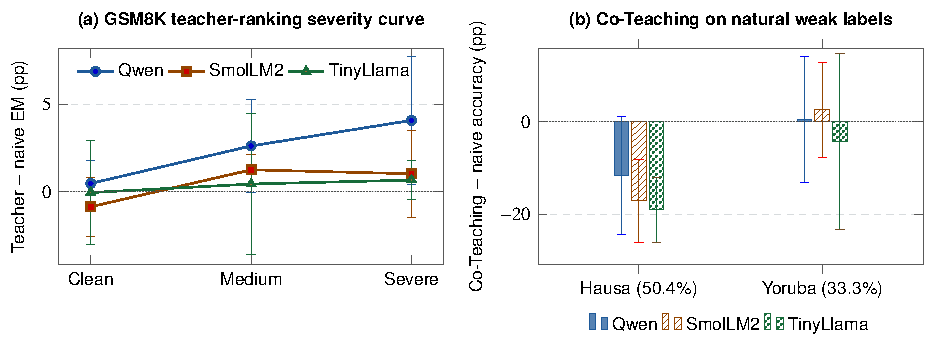
\includegraphics[width=\textwidth]{figures/evidence.pdf}
\caption{Paired mean changes with descriptive 95\% Student-\(t\) intervals
over three seeds; intervals describe seed variation only.  (a) Teacher ranking trends upward with GSM8K contamination,
but none of nine jointly corrected contrasts is significant.  (b) Oracle-rate
Co-Teaching is uniformly harmful on higher-noise Hausa and mixed on lower-noise
Yoruba; both frozen development gates fail and neither clean test split is
evaluated.}
\label{fig:evidence}
\end{figure*}

\subsection{Cost}
In a concurrently executed, matched 64-question diagnostic, teacher ranking costs \(1.52\times\)
the naive SmolLM2 wall time and \(1.58\times\) the naive TinyLlama time.
Serial scoring of 256 candidates takes approximately 8.1 seconds and the
teacher path peaks at 5.57 GiB allocated GPU memory; these are environment-
specific diagnostics, not isolated throughput measurements.

\section{Discussion}
Across the two server tasks, canonical-probability exchange is compatible by
construction but has no consistent accuracy benefit: the tested pipeline is
harmful on AG News, while the TREC effect is inconclusive and its interval
spans modest harm and benefit.  Both tasks show lower observed 10-bin ECE, a
secondary pattern that motivates a dedicated calibration study.
The post-primary TREC decomposition further rejects a simple explanation in
which contamination makes client probabilities harmful and routing repairs
them: severe uniform transfer has the highest accuracy, whereas routing trades
away that gain while lowering descriptive NLL and ECE.
Function-space compatibility is therefore necessary but insufficient for
accuracy gains.  The Qwen result is consistent
with the hypothesis that a clean training-only reference ranks conflicting
supplied answers better than the unadapted client's own loss; the present
experiments do not establish this mechanism across families.  Cross-family
estimates point in the same direction but are too uncertain to support a
universal claim.

\paragraph{Three distinct failure modes.}
First, LoRA factors from different architectures lack a shared parameter
coordinate system; function-space exchange resolves this interface failure.
Second, canonical probabilities can encode task- and metric-dependent utility:
the same transfer pipeline can lose accuracy, gain accuracy, or improve only
calibration depending on its selection policy.  Third,
small-loss or teacher-based selection is distribution- and model-dependent:
Hausa selection collapses, whereas Yoruba purity improves without reliable
accuracy gains.  Conflating these failures can make an aggregation interface
appear robust while leaving knowledge utility untested.

\paragraph{Implication.}
A robust audit should compare an anchor-only server with clean uniform,
contaminated uniform, and routed contaminated arms.  It should distinguish
server-side from end-to-end optimizer work and audit selected composition.
Otherwise, a near-zero net contrast can conceal large opposing mixture and
selection effects, and better calibration can be mistaken for accuracy utility.

Overall, the evidence supports an evaluation contribution rather than a new
federated optimizer.  AG News diagnoses a server-accuracy failure and TREC
shows both an inconclusive net effect and a post-primary selection-induced
accuracy--calibration reversal, while the controlled and natural-label
studies show that established local-selection baselines are not uniformly
robust.  These findings are complementary but concern distinct endpoints;
they do not turn the training-only teacher endpoint into a federated algorithm.

\section{Limitations and Ethics}
Conflicts are controlled synthetic interventions and do not represent all
annotation processes.  The Hausa and Yoruba studies add naturally occurring
weak classification labels but are development-only; naturally occurring numerical
label errors remain untested.  Most comparisons use three seeds, giving
unstable intervals and low power after multiplicity correction.  The
post-observation five-seed AG check strengthens directional consistency but
does not add a new task or untouched test set.  The public-anchor
teacher adds compute and may encode biases from pretraining.  TREC adds an
independently sourced task and five designated official seeds, but its final
protocol followed documented instrumentation repairs, its official test contains only
500 questions, its published license is recorded as unknown, and language-model
pretraining contamination cannot be ruled out.  The ten-seed decomposition was
designed after that test and its primary aggregate had been observed; corrected
contrasts on the reused test are mechanistic, not independent confirmation.
The severe arm jointly changes conflict and off-task content, so its
\(1.58\pp\) effect cannot be assigned to either component or generalized to
natural corruption.  Neither logits,
losses, nor anchors provide formal privacy; membership or reconstruction
leakage is not measured.  We make no privacy-preserving, production, or broad
generalization claim.  FedClean and Delora are not directly applicable to the
open-answer heterogeneous interface, but we have not shown that our endpoint
outperforms them in their native homogeneous classification setting.

\paragraph{AI-assistance disclosure.}
OpenAI Codex assisted with code drafting, experiment orchestration, artifact
validation, and manuscript editing.  The human authors are responsible for
the study design and submission, verified the cited sources and reported
results against the raw artifacts, and take full responsibility for the
paper's content.

\section{Reproducibility}
The artifact includes hashed manifests, serialized JSON run protocols, exact
model weight hashes, per-run raw records, deterministic mixture construction,
generated Markdown summaries, and unit tests.  The official-test and
secondary-holdout records are explicitly distinguished.  The paper tables are
derived from source records rather than manually entered experiment logs.
Because these artifacts are currently workspace files rather than an external
timestamped preregistration, their hashes establish internal consistency, not
independent proof of creation time.  A sidecar clarification records the
natural-noise oracle-rate use without rewriting its original protocol.
The primary TREC schema embeds protocol, runner, task-core, model, data, split,
argument, mixture, simplex, and wire-payload hashes and is checked as a full
5-by-2 matrix.  The post-primary TREC artifact separately checks a complete
10-by-4 matrix, three frozen adjacent contrasts, invalidated instrumentation
history, and final summarizer/verifier hashes.  The legacy AG/GSM record schema does not embed the protocol digest, complete
CLI, or every evaluation-file hash; current verifiers therefore establish
artifact consistency but not independent historical provenance.
The runtime exposed one device labeled NVIDIA GeForce RTX 4090 with 49,140 MiB
visible memory; this host-reported capacity is not a claim about retail-device
specifications.  Experiments used Linux 6.8 with Python 3.10.20, PyTorch 2.11.0+cu128, Transformers 4.57.6,
PEFT 0.18.1, and SciPy 1.15.3.  Primary comparisons use three explicitly
recorded seeds; primary TREC uses five seeds, its disclosed post-primary
ablation ten new seeds, and the AG post-observation check five separately
reported seeds.  Protocol files contain the final optimizer, batch, LoRA, and generation
settings.

\bibliography{references}
\end{document}
